\question Java manages memory for the programmer (this is why it is considered a ``high-level" language). If you have worked with ``low-level" languages such as C/C++, perhaps you understand both the freedom and pain that comes with allocating and de-allocating memory on your own. Java programmers greatly benefit from this abstraction, but let's understand how and why this works.


This diagram depicts the memory layout for all processes in UNIX systems.
\begin{center}
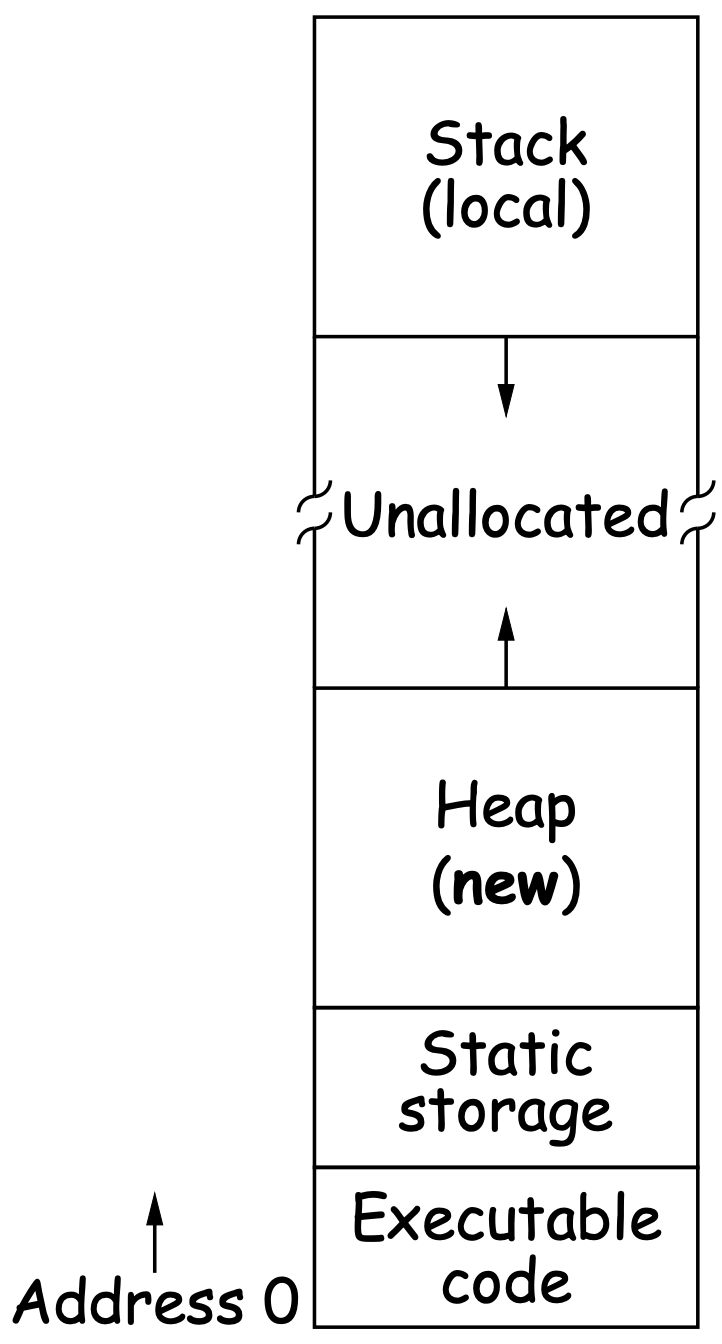
\includegraphics[scale=0.3]{unix-memory.png}
\end{center}
Let's first discuss how each memory region is allocated. The executable file is stored at the lowest address. This region is read-only and is initialized when the process is created and given a program to execute. Global and static variables are stored in static storage. Space for this region is allocated at compile time. All objects created with the \texttt{new} keyword in Java are stored in the heap. Heap memory is \textit{dynamically allocated} at runtime. All local variables used within functions are stored in the stack. Stack space is also allocated at compile time.

De-allocation, also known as \textit{garbage collection}, is the more complicated question. During a process's lifetime, it will allocate and use memory. After a variable's last access (before the process dies), the memory that it occupies must be freed to make space for additional memory that the process may use. Determining \textit{when} de-allocation should occur is the million dollar question.

The executable code isn't de-allocated until the process is finished executing (to do so would be like pulling a rug from under your feet). Data in static storage persists throughout the process's entire lifetime. Stack variables are automatically allocated and de-allocated (the code for this is created during compilation).

In this class, we introduce methods for the de-allocation of heap memory. Since it has been dynamically allocated at runtime, we must also garbage collect at runtime. This worksheet will discuss \textbf{Free List}, \textbf{Mark and Sweep}, and \textbf{Reference Counting}. If you find garbage collection particularly interesting, you should look into exciting careers at Waste Management of Alameda County and/or take CS 164.

\ifprintanswers\else
\begin{lstlisting}

\end{lstlisting}
\fi

\begin{solution}
\begin{lstlisting}

\end{lstlisting}
\end{solution}